
% \begin{abstract} The Suffix Array (SA) is a fundamental data structure
% which is widely used in the applications such as string matching, text
% index and computation biology, etc. How to sort the suffixes of a string in
% lexicographical order is a primary problem in constructing SAs, and
% one of the widely used suffix sorting algorithms is
% \emph{qsufsort}. However, \emph{qsufsort} suffers one critical
% limitation that the order of suffixes starting with the same $2^k$
% characters can not be determined in the $k$-th round. To this point,
% in our paper, an efficient suffix sorting algorithm called
% \emph{dsufsort} is proposed by overcoming the drawback of the
% \emph{qsufsort} algorithm. In particular, our proposal maintains the
% \emph{depth} of each unsorted portion of SA, and sorts the suffixes
% based on the \emph{depth} in each round. By this means, some suffixes
% that can not be sorted by \emph{qsufsort} in each round can be sorted
% now, as a result, more sorting results in current round can be
% utilized by the latter rounds and the total number of sorting rounds
% will be reduced, which means \emph{dsufsort} is more efficient than
% \emph{qsufsort}. The experimental results shows the effectiveness of
% the proposed algorithm, especially for the text with high repetitions.
% \end{abstract}

\chapter{一种高效的后缀排序算法}
\section{引言}
\label{sec:introduction}

如何将给定字符串的所有后缀按照字典序进行排序, 是构建后缀数组的主要问
题。 目前, \emph{qsufsort}\cite{Larsson2007} 算法是解决该问题广泛使用的
算法之一。 该算法采用“前缀倍增”技术对后缀进行逐轮排序, 每一轮的排序将
基于上一轮的结果, 直到所有后缀都处于正确的字典序。 具体地, 首先所有后缀
将根据其首字符进行排序, 然后在每一轮中, 排序所依据的字符数将翻
倍, 这样, 在第\emph{k}轮之后, 所有后缀将根据其前 $2^{k}$ 个字符进行排
序。 这也意味着, 对于那些前$2^{k}$字符相同的后缀, 它们的次序无法在
第$k$轮之后被确定。 因此, 对于那些具有较大 \emph{LCP}(Length of the
Longest Common Prefix)的后缀, \emph{qsufsort} 需要许多轮才能确定它们的
次序, 这会严重影响算法效率。

为了克服 \emph{qsufsort} 的这种缺陷, 在本章中, 将提出一种基
于 \emph{qsufsort} 算法的改进的后缀排序算法--\emph{dsufsort}。 其核心思
想在于, 对后缀数组SA中每一个还未排序的部分(称作一个“桶”(bucket)),
\emph{dsufsort} 算法将记录该桶中所包含后缀(已知的)最大的\emph{LCP} (称
为该桶的“深度”), 并且在运行过程中对其进行实时更新。 然后, 在每一轮中,每
一个未排序桶中的后缀, 将基于该桶的深度进行排序。 通过这种方式, 许多后缀
在第$k$轮中, 可以基于超过前$2^k$个字符进行排序。 这意味
着, 在第$k$轮中, 无法由\emph{qsufsort}算法确定顺序的那些前$2^{k}$字符相
同的后缀, 有可能在$k$轮中被确定顺序。 由于在每轮中有更多的后缀能够被排
序, 因此有更多的排序结果可以被后面的过程所利用, 这会减少总共所需要的轮
数。 因此, \emph{dsufsort} 比 \emph{qsufsort} 更加高效, 尤其对于拥有较
大 \emph{LCP} 的后缀。

本章内容组织如下: 第2节介绍相关工作。 第3节将给出所用的符号和术语。
\emph{qsufsort} 和改进的 \emph{dsufsort} 算法将在第4节中进行详细介
绍。 第5节将讨论一些高效的实现技术。 第6节进行实验对比。 第7节是对本章进行
总结。

\section{相关工作}

在过去的二十年中, 大量的具有不同时间和空间复杂度的后缀数组构建算法(即后
缀排序算法) 被提出。 接下来, 将对其中的一些算法进行简要地回顾, 对其更详
细的介绍, 可参考综述文献 \cite{Puglisi2007} \cite{Dhaliwal2012}。

从后缀树来构造后缀数组, 是构建后缀数组最简单的方法之一, 其主要缺陷在于
过高的空间和和时间开销。 Manber 和 Myers \cite{Manber1993} 第一个提出了
直接构建后缀数组的算法, 其时间复杂度为 $O(nlogn)$ (其中$n$是给定字符串
的长度)。 该算法使用了一种被称为“前缀倍增”的技术(最早来源于Karp
\cite{Karp1972}): 首先, 后缀将按照其首字符进行排序, 接着在之后的每一轮
中, 将按照加倍长度的前缀对后缀进行排
序。Larsson和Sadakane\cite{Larsson2007} 提出了 \emph{qsufsort} 算法
对Manber的算法进行改进。 与Manber算法在每一轮中都需要检查SA中所有的桶不
同, \emph{qsufsort} 算法会标记那些之前已经被排过序的桶。 这样, 在每轮中
它将跳过那些被标记的桶, 只对未排序的桶进行排序。 尽管在理论上,
\emph{qsufsort} 算法和Manber的算法具有相同的时间复杂度, 在实际当中,
\emph{qsufsort}算法要高效得多。 Schurmann\cite{Schurmann2007} 提出了一
种具有 $O(n^2)$ 时间复杂度的方法-- \emph{bpr}。 与Manber算法
和 \emph{qsufsort} 算法在每一轮中使用广度优先策略来对每一个桶进行排序不
同, \emph{bpr} 使用了深度优先的排序策略: 对于每一个未排序的桶, 它将递归
地对其中的后缀进行排序, 直到所有后缀都完全有序。  Rajasekaran
\cite{Rajasekaran2014} 提出了被称为 \emph{RadixSA} 的新算法, 该算法具
有 $O(nlogn)$ 的时间复杂度。 与前面三个算法使用简单的从左到右的顺序来对
桶进行排序不同, \emph{RadixSA} 使用了特殊的排序顺序: 假设第$i$个后
缀 $S_i$ 处于桶$B_i$中, 那么算法将首先对桶 $B_n$ 进行排序, 然后依次对
桶 $B_{n-1},\,\dots,\, B_1$ 进行排序。 这种顺序确保了在对桶 $B_i$ 排序
之后, 后缀$S_i$ 已经处于其在SA中的最终位置。

Seward \cite{Seward2000} 提出了另外两个后缀排序算法:
\emph{Copy} 和 \emph{Cache}。 它们首先将基于后缀的前两个字符对其进行排
序, 然后按照由小到大的顺序(即根据桶中所包含后缀的多少,由少到多)对未排
序的桶进行排序, 一旦一个桶完全有序, 排序的结果将被后续过程使用。 然而,
\emph{Copy} 和 \emph{Cache} 使用相同的函数对所有后缀进行排序, 这对具有
很长公共前缀的后缀(即具有较大$LCP$的后缀)效率不高。 为解决此问题,
Manzini \cite{Manzini2004} 提出了被称为 \emph{deep-shallow} 的算法。 当
对一个桶进行排序时, \emph{deep-shallow} 会使用\emph{shallow} 排序函数对
具有较短公共前缀的后缀进行排序, 而使用 \emph{deep} 排序函数对具有较长
公共前缀的后缀进行排序。 尽管 \emph{deep-shallow} 在理论上有良好的性能,但
复杂的框架限制了它在实际当中的使用。

以上所介绍的算法都具有超线性的时间复杂度。 然而, 已经有线性时间复杂度的
算法被提出,比较知名的包括 \emph{KA} \cite{Ko2005}, \emph{KS}
\cite{Karkkainen2006} 和 \emph{KSP}\cite{Kim2005} 算法。 \emph{KSP} 算法
采用了和Farach算法 \cite{Farach1997} 类似地归并策略。 \emph{KS} 算法使
用了分而治之的策略,包含3步: (1) 递归地为那些起始于位置 $i$ ($i~mod~3
\neq 0$) 的后缀构造后缀数组; (2) 使用第一步的排序结果,为那些剩余后缀
构建后缀数组; (3) 将第一步和第二步中构建的后缀数组合并为一个。
\emph{KA} 算法是 \emph{two-stage} 算法\cite{Itoh1999} 的一个改进, 它将
字符串中的所有后缀分成两类:L-类和S-类。 然后递归地对所有L-类后缀进行排
序,之后,S-类后缀的顺序可由L-类后缀的顺序诱导得到。 Nong
\cite{Nong2011}提出了两个算法 \emph{SA-IS} 和 \emph{SA-DS} 来改
进 \emph{KA} 算法。 它们分别使用了“变长最左S-类子串”和“定长d-关键子
串”来对问题进行规约, 同时使用了简单高效的算法对这些采样子串进行排
序。 最近, Nong\cite{Nong2013} 针对常量字符集又提出了一个线性时间算
法--\emph{SACA-K}, 该算法仅需要 $O(1)$ 大小的工作空间。 尽管线性时间算法
在理论上具有较好的时间复杂度,但在实际应用中, 它们的性能却常常不如在实
现方面经过高度优化过的超线性算法 \cite{Rajasekaran2014}。

目前, 有许多外存算法\cite{Karkkainen2014,Nong2014,Nong2015} 被提出用于
构建较大的后缀数组,外存算法所需要的空间主要由价格低廉且空间巨大的磁盘来
提供。 通过使用外存算法,可以构造出那些无法放入内存的巨大后缀数组。 为
了进一步加快排序速度,有许多学者提出了如何并行地构建后缀数
组 \cite{Schmidt2016,Metwally2016,Flick2015,Deo2013}.

\section{相关概念}
\label{sec:stucture}

令 $\Sigma$ 表示有限个字符组成的\emph{字符集} (本章只关注于ASCII字符
集, 即 $|\Sigma| = 256$ 且每个字符占用一个字节的存储空间)。 给定字符
集$\Sigma$, $\Sigma$ 上的字符串及其子串定义如下:

\textbf{定义 1.} $\Sigma$ 上的\emph{字符串}是由有限个 $\Sigma$ 中的字符
组成的序列。 $\Sigma$ 上长为$n$的字符串可表示为: $T =
t_0t_1..t_{n-1}$, 其中 $T[i] = t_i \in \Sigma$ $(0 \leq i \leq
n-1)$。$T$ 上的一个\emph{子串}是由 $T$ 中任意个连续字符所构成的字符
串。 $T$中, 起始于位置 $i$ 且终止于位置 $j$ 的子串可表示 $T[i,j]$。

在后缀排序中,最基本的概念是后缀和前缀,它们都是给定字符串特殊的子串,
定义如下:

\textbf{定义2.} 对于字符串 $T = t_0t_1..t_{n-1}$, 其起始于位置
$i(0 \leq i \leq n-1)$ 的\emph{后缀}是子串 $T[i,n-1]$, 由$S_i(T)$表
示。  $T$ 的长为 $h$ 的\emph{前缀}是子串 $T[0,h-1]$, 由 $P_h(T)$ 表示。

在本章中, 当提及某些后缀时, 它们一定是关联于同一个字符串的,所以符
号 $S_i(T)$ 可以无歧义地简写成 $S_i$。 为了确保没有后缀是其它某个后缀的
前缀, 通常会向字符串 $T$ 的末尾插入一个特殊字符 '\$', '\$' 被定义为在字
典序上小于任何 $\Sigma$ 中的字符。 使用表达式 $S_i \prec S_j$ 来表示后
缀 $S_i$ 以字典序小于后缀 $S_j$。 且我们的最终目标是, 将给定字符串的所
有后缀按照字典序由小到大进行排序, 形成后缀数组:

\textbf{定义 3.} 给定字符串 $T = t_0t_1..t_{n-1}\$$,
$T$ 的\emph{后缀数组}(SA)是一个具有 $n+1$ 个元素的数组 $SA[0 \dots
n]$, 其元素是 $0 \sim n$ 的整数, 使得对于任意 $0 \leq i < j \leq n$, 都
有 $S_{SA[i]} \prec S_{SA[j]}$。

由于一个后缀可以唯一地由其起始位置确定, 只需要在SA中存储后缀的起始位置。
为了简单起见, 术语“(后缀的)次序”如果不做特殊说明, 将总是代表字典
序。 基于字典序, 可以通过只比较后缀的前$h$个字符, 来进一步定义后缀
的 \emph{h-序}: $S_i$ 被称为 \emph{h-小于} $S_j$ 当且仅当 $P_h(S_i)
\prec P_h(S_j)$, 这种关系被表示为 $S_i \prec_h
S_j$。  同理, 符号 $=_h$ 和 $\preceq_h$ 可以被类似地定义。 明显地, 有:
$S_i \prec_h S_j \Longrightarrow S_i \prec S_j$。 如果所有的后缀都都依
据其前 $h$ 个字符被排好序, 则它们被称为是\emph{h-有序}的。

接下来将介绍“桶”(bucket)的概
念, 它是 \emph{qsufsort} 和 \emph{dsufsort} 算法中的核心概念。

\textbf{定义 4.} 给定后缀数组SA, SA上一个深度为$h$的\emph{桶}, 是一个子
数组 $SA[l \dots r]$ $(l \leq r)$, 满足:
$S_{SA[l]} =_h S_{SA[l+1]}\dots =_h S_{SA[r]}$ 且
$S_{SA[l-1]} \neq_h S_{SA[l]}$ 及 $S_{SA[r]} \neq_h
S_{SA[r+1]}$。 桶 $SA[l \dots r]$ 的序号被定义为 $l$, 该桶被表示
为 $B_l$。

注意, 深度 \emph{h} 是桶 $B_l$ 中所包含后缀\emph{当前已知的}公共前缀的
长度。 为了记录每一个后缀所在的桶, 使用一个数组 $B$: 若 $B[i] =
j$, 则 $S_i$ 当前处于桶 $B_j$ 中。 注意区别: $B_i$ 是编号为 $i$ 的桶,
而 $B[i]$ 是后缀 $S_i$ 当前所在桶的编号。

给定后缀 $S_i$ 和 $S_j$, $LCP(S_i, S_j)$ 被定义为 $S_i$ 和 $S_j$ 最长公
共前缀的长度。 基于 $LCP(S_i, S_j)$, 字符串的平均 \emph{LCP} 可以按如下
定义:

给定长为$n+1$的字符串 $T$ 及其后缀数组 $SA$, $T$ 的平均$LCP$由以下公式
计算:

\begin{equation}
\frac{1}{n}\sum_{i=0}^{n-1}LCP(S_{SA[i]},S_{SA[i+1]}).
\end{equation}

字符串的平均$LCP$, 可以粗略地估计对该字符串后缀进行排序所需的计算量: 如
果平均$LCP$较大, 原则上我们将需要比较更多的字符来确定两个后缀的顺序。

\section{ \emph{dsufsort} 算法}

本节将介绍基于 \emph{qsufsort} 算法的改进的后缀排序算
法---\emph{dsufsort}。 \emph{dsufsort} 通过在排序过程中实时地维护每个桶
的深度来提高 \emph{qsufsort} 算法的效率。 当对某个桶进行处理时, 将根据
桶的深度对其中的后缀进行排序。 通过这种方式, 相比 \emph{qsufsort} 算法,
\emph{dsufsort} 算法在每一轮中可以确定更多后缀的顺序, 换言之, 对所有后
缀进行排序, \emph{dsufsort} 算法将需要较少的轮数, 这能够减少算法的运行
时间, 提高算法效率。 接下来, 先简要地介绍 \emph{qsufsort} 算法的核心思
想, 然后详细地讨论对其的改进算法 \emph{dsufsort}。

\subsection{ \emph{qsufsort}算法简介}
\label{sec:qsufsort}

Larsson和Sadakane所提出的 \emph{qsufsort} 算法使用了被称为“前缀倍
增”的技术来对后缀进行逐轮排序。 在第0轮中, 给定字符串的所有后缀将根据
其首字符进行排序。 之后, 所有具有相同首字符的后缀都会被排列到一起形
成$SA$上一个深度为1的桶, 而整个 $SA$ 将(在逻辑上)被划分为一系列的深度
为1的桶: 第一个桶中所包含的后缀具有最小的首字符, 第二个桶中所包含的后缀
具有次小的首字符, .... 依此类推。

注意, 如果一个深度为1的桶只包含一个后缀, 该桶及其包含的单个后缀被称为
是\emph{完全有序的}, 因为该后缀可以根据首字符将其从其它后缀中区分出来,
它已经处于SA的最终位置, 将来无需再对其进行排序。 然而, 如果一个深度为1的
桶包含了超过一个后缀, 该桶及其所包含的后缀则被称为是\emph{未排序的}, 后
续将需要比较更多的字符来确定其后缀的顺序。

在第0轮后, 所有后缀都处于\emph{1-有序}的状态。 并且不失一般性地, 任意两
个后缀 $S_i$ 和 $S_j$ 的1-序可由其所在桶的序号确定:
$S_i \preceq_1 S_j \iff B[i] \leq B[j]$。

通过使用前缀倍增技术, 在每轮过后, 所有的后缀都将基于其倍增长度的前缀被
排序。 这样, 在第 \emph{k-1} 轮之后, 所有的后缀都将处于 $2^{k-1}$-有序,
换言之, 所有未排序的桶都有同样的深度 $2^{k-1}$, 且这些未排序的桶, 将在
第$k$轮中被从左到右逐个进行排序。

现在, 假设未排序的桶 $B_p$ 即将在第 $k$ 轮被排序。 对 $B_p$ 中任意
的 $S_j$ 和 $S_i$, 由于 $S_i =_{2^{k-1}} S_j$, $S_i$ 和 $S_j$ 之间的次
序将依赖于 $S_{i+2^{k-1}}$ 和 $S_{j+2^{k-1}}$ 的次序, 即:
$S_i \prec S_j \iff S_{i+2^{k-1}} \prec S_{j+2^{k-1}}$。 这里,
$S_{i+2^{k-1}}$($S_{j+2^{k-1}}$) 被称作 $S_i$($S_j$) 的锚后缀。 然而,由
于当前仅能够确定 $S_{i+2^{k-1}}$ 和 $S_{j+2^{k-1}}$ 的 $2^{k-1}$-序, 相
应地,也仅能够确定 $S_i$ 和 $S_j$ 的 $2^k$-序:
$S_i \preceq_{2^k} S_j \iff S_{i+2^{k-1}} \preceq S_{j+2^{k-1}} \iff
B[i+2^{k-1}] \leq B[j+2^{k-1}]$。  这种等价关系说明了如何在第 $k$ 轮中,
将 $B_p$ 中的后缀排成 $2^k$-有序的: 首先,对于 $B_p$ 中任一后缀 $S_i$,
将其锚后缀所在的桶序号,即 $B[i+2^{k-1}]$ 作为 $S_i$ 的键值: $key(S_i)
= B[i+2^{k-1}]$, 然后,使用普通的整数排序算法对所有的键值进行排序,接着
将 $B_p$ 中的后缀,依据其键值的整数序进行重新排序,之后,$B_p$ 中的后缀
将处于 $2^k$-有序。

一旦某个未被排序的桶被处理过, 将会根据以下两种情况产生新的桶: 1) 如果
某个后缀具有唯一的键值, 那么它将处于SA的最终位置,并独自形成一个完全有
序的(包含单个后缀的)桶。 2) 如果某些后缀具有相同的键值, 那么它们将被排列
在一起形成一个新的未排序的桶,并将在后续过程中进一步对其排序。 另
外,$B$ 数组也需要根据新产生的桶做出相应的更新。

\emph{qsufsort} 算法逐轮地对未排序的桶进行排序,直到所有后缀都被完全有
序。注意, 通过使用前缀倍增技术, 确定每个后缀次序所依据的前缀将会在每一
轮后倍增,所以,对长为$n$的字符串,其任意两个后缀的次序都可以在最
多 $logn$ 轮后被确定。

\subsection{dsufsort 算法: 记录并维护每一个未排序桶的深度}
\label{sec:dsufsort}

如前所述, 在第 $k$ 轮中, \emph{qsufsort} 算法将依据每个后缀前 $2^k$个字
符对其进行排序, 这意味着, 对于那些前$2^k$个字符都相同的后缀, 该算法无
法在第 $k$ 轮中确定其次序。 因此,对于具有很长公共前缀的后
缀, \emph{qsufsort} 需要许多轮才能确定其次序,这会严重影响算法效率。

为了提升算法性能,在每一轮中,应依据尽可能多的(前缀)字符来对后缀进行排
序。 为此, 对每一个未排序的桶, \emph{dsufsort} 算法将维护其桶的深度 (即
当前已知的,桶中后缀的最长公共前缀的长度), 并在每一个桶被处理后,对其深
度进行更新。 在每轮中, 当对某个桶中的后缀进行排序时, \emph{dsufsort}
算法将使用桶的深度来计算其后缀的键值, 然后对其进行排序。 在第$k$轮中,
通过使用基于桶深度计算得到的键值, 对于某些后缀,可以依据多于$2^k$个前缀
字符来对其进行排序, 这样, 一些前 $2^k$ 字符都相同的后缀,便可以在
第 $k$ 轮中确定其次序。 相比\emph{qsufsort}算法, \emph{dsufsort} 算法在
每轮中可以确定更多后缀的次序, 因此,需要更少的轮数来完成排序任务。

为了记录桶的深度, 使用一个数组 $D$,使得每个桶的深度可以由其编号索引得
到: 对于桶 $B_p$, 它的深度为 $D[p]$。 在第0轮后, 对每一个新产生的
桶 $B_p$,令 $D[p] = 1$。

类似于 \emph{qsufsort}, \emph{dsufsort} 算法逐轮地对后缀进行排序, 直到
所有后缀都完全有序。 在每轮中, \emph{dsufsort} 算法采用了两阶段的“排序-更
新” 策略来处理未排序的桶及更新其深度信息。 举例说明, 假设桶 $B_p$ 即将
在第$k$轮中被处理:

\begin{itemize}
\item \textbf{排序:} 不失一般性地, 对 $B_p$ 中的任意 $S_i$ 和 $S_j$, 由
  于 $S_i =_{D[p]} S_j$, $S_i$ 和 $S_j$ 之间的次序将取决
  于 $S_{i+D[p]}$ 和 $S_{j+D[p]}$ 之间的次序:
  $S_i \prec S_j \iff S_{i+D[p]} \prec S_{j+D[p]} \iff B[i+D[p]] <
  B[j+D[p]]$。 其中 $S_{i+D[p]}$($S_{j+D[p]}$) 是 $S_i$($S_j$) 的锚后
  缀。 根据以上等价关系, 对任意 $B_p$ 中的 $S_i$ , \emph{dsufsort} 算法
  将使用 $B[i+D[p]]$ (而非 \emph{qsufsort} 使用的 $B[i+2^{k-1}]$) 作为
  它的键值, 并使用普通的整数排序算法, 对所有后缀的键值进行排序。 然后,
  根据键值的(算术)顺序, 对 $B_p$ 中的后缀进行重新排序。

  现在, $B_p$中的每个 $S_i$, 都根据其前 $D[p] + D[B[i+D[p]]$ 个字符(而
  非前 $2^k$ 个字符)被排序。 稍后将看到, 在第 $k$ 轮中 (即在 \emph{k-1}
  轮之后), 一定有: $D[p] \geq 2^{k-1}$ 且 $D[B[i+D[p]] \geq 2^{k-1}$,
  这意味着, 所有后缀将根据其前至少$2^k$个字符进行排
  序, 这样 \emph{dsufsort} 的性能至少和 \emph{qsufsort} 持平。 同时也将
  看到, 在某些时刻, 存在 $D[p] > 2^{k-1}$ 的情况, 这意味着 $B_p$ 中的所
  有后缀将基于超过前 $2^k$ 个字符进行排序, 此时, \emph{dsufsort} 要优
  于 \emph{qsufsort}。

\item \textbf{更新:} 当$B_p$ 被处理之后, 数组 $D$ 和 $B$ 将立刻被更新。
  假设根据键值大小:
  $key(S_{i_1}) \leq key(S_{i_2}) \leq \dots \leq key(S_{i_s})$, 后缀被
  重排为 $S_{i_1}, S_{i_2},\dots,S_{i_s}$。 根据其键值是否唯一,可将后缀
  分为两类:

\begin{itemize}

\item 对任意 $S_{i_j}$ 满足 $key(S_{i_{j-1}}) \neq
  key(S_{i_j})$ 且 $key(S_{i_j}) \neq key(S_{i_{j+1}})$, $S_{i_j}$ 将处
  于其在SA中的最终位置, 同时构成一个完全有序的单元素桶:
  $B_{p+j-1}$。 $S_{i_j}$ 所在的桶, 将相应地被更新为: $B[i_j] = p+j-1$。
  然而, 无需更新已经完全有序的桶的深度(即无需更新$D$数组)。

\item 对每一组后缀 $\{S_{i_l}, S_{i_{l+1}},\dots,S_{i_r}\}$ 满足:
  $key(S_{i_l}) = key(S_{i_{l+1}}) = \dots = key(S_{i_r}) = m$,
  $key(S_{i_{l-1}}) \neq m$ 且 $key(S_{i_{r+1}}) \neq m$, 该后缀
  组 $\{S_{i_l}, S_{i_{l+1}},\dots,S_{i_r}\}$ 将构成一个新的未排序桶:
  $B_{p+l-1}$。 由于 $B_{p+l-1}$ 中每个后缀的锚后缀都在桶 $B_m$ 中,
  $B_m$ 被称为是 $B_{p+l-1}$ 的"锚桶"。 该组中所有后缀所在的桶也将被相应
  地更新: 每一个 $B[i_l], B[i_{l+1}], \dots, B[i_r]$ 都将被更新
  为 $p+l-1$。  由于已经知道:
  $S_{i_l} =_{D[p]} S_{i_{l+1}} =_{D[p]} \dots =_{D[p]}
  S_{i_r}$ 及
  $S_{i_l+D[p]} =_{D[m]} S_{i_{l+1}+D[p]} =_{D[m]} \dots =_{D[m]}
  S_{r+D[p]}$, 所以有:
  $S_{i_l} =_{D[p]+D[m]} S_{i_{l+1}} =_{D[p]+D[m]} \dots =_{D[p]+D[m]}
  S_{i_r}$。  因此, 新产生桶 $B_{p+l-1}$ 的深度应为: $D[p+l-1] = D[p] +
  D[m]$, 我们使用该等式来设置新的未排序桶的深度。
\end{itemize}

\end{itemize}


基于两阶段的\emph{排序--更新}策略, \emph{dsufsort} 算法的框架可以总结如
下:

\begin{itemize}

\item \textbf{步骤 1.} 初始化(第0轮): 根据首字符, 对输入字符串的所有后缀
  进行排序。 对每一个新产生的未排序桶 $B_p$, 令 $D[p] = 1$, 且对 $B_p$
  中的任一 $S_i$, 令 $B[i] = p$。

\item \textbf{步骤 2.} 对SA中每一个未排序的桶 (比如 $B_p$), 执行以
  下\emph{排序--更新}操作:

\begin{enumerate}
\item \emph{排序}: 对 $B_p$ 中的每个后缀 $S_i$, 令 $B[i+D[p]]$ 作为它的
  键值, 并使用整数排序算法, 对所有后缀的键值进行排序, 再根据键值大小,
  对 $B_p$ 中的后缀进行由小到大排序。
\item \emph{更新}: 假设 $B_p$ 中的后缀被排序为: $S_{i_1},
  S_{i_2},\dots,S_{i_s}$。 对任意 $S_{i_j}$ 满足:
  $key(S_{i_{j-1}}) \neq key(S_{i_j})$
  且$key(S_{i_j}) \neq key(S_{i_{j+1}})$, 将 $B[i_j]$ 设置
  为 $p+j-1$。 对每一组后缀 $\{S_{i_l}, S_{i_{l+1}},\dots,S_{i_r}\}$ 满
  足: $key(S_{i_l}) = key(S_{i_{l+1}}) = \dots = key(S_{i_r}) = m$,
  $key(S_{i_{l-1}}) \neq m$ 且 $key(S_{i_{r+1}}) \neq m$, 产生一个新的
  未排序桶 $B_{p+l-1}$。 将 $D[p+l-1]$ 设置为 $D[p] + D[m]$, 同时将每一
  个 $B[i_l], B[i_{l+1}], \dots, B[i_r]$ 设置为 $p+l-1$。
\end{enumerate}

\item \textbf{步骤 3.} 如果SA中没有未排序的桶, 则算法结束; 否则, 跳转
  到 步骤 2 并开始新的一轮排序。

\end{itemize}

如前所述, \emph{dsufsort} 算法具有如下重要性质:


\textbf{性质.} \emph{对第$k$ \emph{(}$k = 0,1,2,\dots$ \emph{)} 轮中产
  生的每一个未排序的桶 $B_q$, 都有 $D[q] \geq 2^k$。}


\textbf{证明:} 由归纳法可证。 首先, 对于任何第0轮中产生的未排序
桶 $B_q$, 都有 $D[q] = 1 \geq 2^0$。  然后, 假设 $B_q$ 是第 $k$ 轮中产
生于 $B_p$ 的新的未排序桶, 且 $B_m$ 是 $B_q$ 的锚
桶。 由于 $B_p$ 和 $B_m$ 是产生于第$k-1$ 轮的未排序桶, 由归纳假设有:
$D[p] \geq 2^{k-1}$ 且 $D[m] \geq 2^{k-1}$, 因此
$D[q] = D[p] + D[m] \geq 2^{k-1} + 2^{k-1} = 2^k$。


该性质确保了 \emph{dsufsort} 算法的性能至少和 \emph{qsufsort} 持平。 然
而, 有必要探讨在何种情形, \emph{dsufsort} 在性能上优
于 \emph{qsufsort}, 更具体地, 何时会出现 $D[q] > 2^k$。 假设当前处于
第 \emph{k-1} 轮, 正在处理第 $k-2$ 轮产生的未排序桶 $B_p$ 且有 $D[p] =
2^{k-2}$。 如果一个新的未排序桶 $B_q$ 产生于 $B_p$ 且其锚桶为 $B_m$, 则
有 $D[q] = D[p] + D[m]$。

关键在于, 如果 $B_p$ 的锚桶 $B_m$ 也是先前在第 $k-1$ 轮中产的新的未排
序桶, 根据刚才证明的性质, 一定有 $D[m] \geq 2^{k-1}$。 所以, 可以得到:
$D[q] = D[p] + D[m] \geq 2^{k-2} + 2^{k-1} > 2^{k-1}$, 这意味着 $B_q$
的深度严格大于 $2^{k-1}$。 因此, 当 $B_q$ 在第 $k$ 轮中被处理时, $B_p$
中的任一 $S_i$ 将会基于其前 $D[p] + D[B[i+D[p]]$ 个字符被排序, 由于
$D[q] > 2^{k-1}$ 且 $D[B[i+D[p]] \geq 2^{k-1}$, $S_i$ 在第$k$轮中将基
于超过 $2^k$ 字符被排序, 这也意味着, \emph{dsufsort} 将优于
\emph{qsufsort}。 更进一步, 如果 $B_m$ 和 $B_q$ 具有相同的情况, 即
$B_m$ 的锚桶同样产生于第 $k-1$ 轮, 则有 $D[m] > 2^{k-1}$。 由于深度的相
互叠加, $D[q]$ 可以远大于 $2^{k-1}$, 因此, 在第$k$轮中, 对$B_q$ 后缀排
序所基于的字符数可以远大于 $2^k$。

\begin{figure}[!h]
\centering
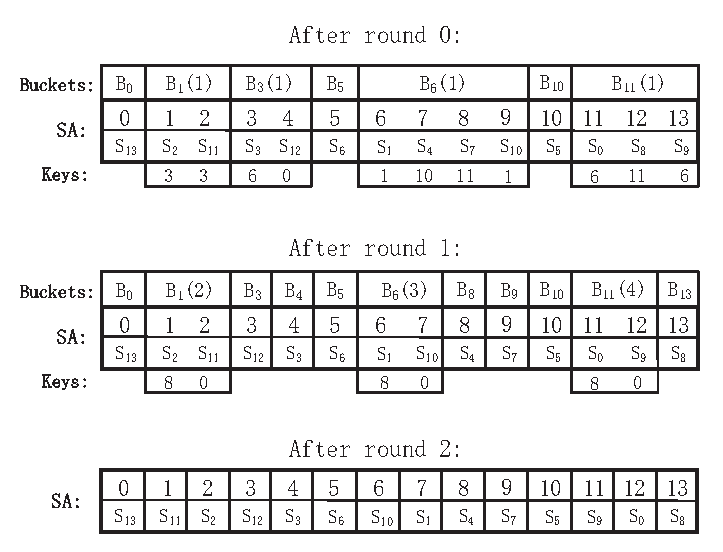
\includegraphics[width=9cm]{figures/3_SS/p1}
\vspace*{8pt}
\caption{使用 \emph{dsufsort} 算法对字符串 '\emph{tobeornottobe}' 的后
  缀进行排序。}
\label{fig:1}
\end{figure}

\textbf{例子.} 图 \ref{fig:1} 说明了使用 \emph{dsufsort} 算法对输入字符
串 $tobeornottobe$ 进行后缀排序的过程。 为了清晰起见, 我们将完整的后
缀 $S_i$ 放入SA中, 而非其起始位置 $i$。 每个桶的深度在其后的括号内显
示。 第0轮过后, 所有后缀都基于其首字符被排序。 由于桶 $B_0$,
$B_5$ 及 $B_{10}$ 都只包含一个后缀, 这三个桶已经完全有序了。

在第1轮中, 产生于第0轮的4个未被排序的桶 $B_1$, $B_3$,
$B_6$ 及 $B_{11}$ 将被依次处理。 将处理 $B_6$ 作为例子, 其余3个桶可以类
似方式处理。 对 $B_6$ 中任一后缀 $S_i$, 其键值可以通过桶的深度来计算:
$key(S_i) = B[i+D[6]]$。 所以, $B_6$ 中所包含后缀的键值分别为:
$key(S_1) = B[1+D[6]] = 1$, $key(S_4) = B[4+D[6]] = 10$,
$key(S_7) = B[7+D[6]] = 11$, $key(S_{10}) = B[10+D[6]] = 1$。 然后, 使用
普通的整数排序函数对这些键值进行排序: $key(S_1) = key(S_{10}) <
key(S_4) < key(S_7)$。  根据键值的大小顺序, $B_6$ 中后缀的 1-序 可以被确
定: $S_1 =_ 1 S_{10} \prec_1 S_4 \prec_1 S_7$。 由于 $S_1$ 和 $S_{10}$
具有同样的键值, 它们将共同构成一个新的未排序桶 $B_6$。 注意, 相比于原先
的(即当前正在被处理的) $B_6$(由 $B_6^{\;old}$ 表示), 新产生
的 $B_6$(由 $B_6^{\;new}$ 表示) 具有相同的桶序号 (这意味
着 $S_1$ 和 $S_{10}$ 所在的桶不变), 但不同的大小和深度。 $B_6^{\;new}$
的深度为 $D[6]^{\;new} = D[6]^{\;old} + D[1] = 3$, 这是因
为 $B_1$是 $B_6^{\;new}$ 的锚桶且 $D[1] = 2$。 另一方面, $S_4$ 和 $S_7$
都具有唯一的键值, 它们将分别构成完全有序的桶 $B_8$ 和 $B_9$, 且仅需要更
新它们所在的桶号: $B[4] = 8$, $B[7] = 9$。 第1轮过后, 将剩余3个未排序的
桶: $B_1^{\;new}$, $B_6^{\;new}$, $B_{11}^{\;new}$。

在第2轮中, $B_1^{\;new}$, $B_6^{\;new}$ 及 $B_{11}^{\;new}$ 将会依次被
处理。 通过使用 $D[1] = 2$, $D[6] = 3$ 及 $D[11] = 4$ 来分别计算后缀的
键值并对其进行排序, 所有3个桶将会在本轮中被完全排序, 算法也随即结束。

为了说明 \emph{dsufsort} 相比于 \emph{qsufsort} 的优势, 考察在第1轮中
对 $B_{11}^{\;old}$ 的处理过程。 由于 $B_{11}^{\;old}$ 中所包含后缀的键
值分别为: $key(S_0)=6$, $key(S_9)=6$, $key(S_8) = 11$, $S_8$ 将构成完全
有序的桶 $B_{13}$, 而 $S_0$ 和 $S_9$ 将构成未排序的
桶 $B_{11}^{\;new}$。 由于 $B_{11}^{\;new}$ 产生于 $B_{11}^{\;old}$, 且
其锚桶为 $B_6^{\;new}$, 因此 $B_{11}^{\;new}$ 的深度为
$D[11]^{\;new} = D[11]^{\;old} + D[6]^{\;new}$。 正如已经知道的,
$B_6^{\;new}$ 同样也产生于第1轮, 且其深度为 $D[6]^{\;new} =
3$, 所以 $D[11]^{\;new} = 1 + 3 = 4$。 因此 $B_{11}^{\;new}$ 的深度大
于2 (在 \emph{qsufsort} 的第1轮中, 所有桶的"深度"都为2)。 这样, 在第2轮
中, $B_{11}^{\;new}$ 中的后缀将至少基于其前 $4+2$ 个字
符 (而非\emph{qsufsort}算法所基于的前 $2+2$ 个字符) 被排序。 其后缀的键
值分别是: $key(S_0)=B[0+D[11] ^{\;new}]=
8$ 和 $key(S_9)=B[9+D[11]^{\;new}]= 13$, 这说明 $B_{11}$ 可以在第2轮中
被完全排序。 相比之下, 在 \emph{qsufsort} 算法中, $B_{11}^{\;old}$ 中后
缀的键值为 $key(S_0) = B[0+2] = 1$ 及 $key(S_9) = B[9+2] = 1$, 这意味
着 $B_{11}^{\;old}$ 无法在第2轮中被完全排序。 所以, \emph{dsufsort} 算法
仅需要3轮便可对所有的后缀完成排序, 而 \emph{qsufsort} 算法则需要4轮。

对于平均LCP较大的输入字符串, \emph{dsufsort}算法所具有的"深度叠加"的特
性将充分发挥, 使其可以更快地确定具有较长公共前缀后缀的次序。


\section{高效的实现}

本节中, 将讨论一些用于提高算法效率的实现技巧。

\subsection{输入变换}

在第0轮中, 所有后缀都将基于其首字符被排序。 实际上, 通过预先对输入字符串
进行变换, 可以使后缀根据前几个字符进行排序。 输入变换包括以下两个步骤:

\subsubsection{字符集压缩}

给定$\Sigma$上的字符串 $T = t_0t_1...t_{n-1}\$$, 令实际出现于$T$ 中的字
符构成有序集 $C = \{c_0, c_1,\dots, c_{m-1}\}$, 其中 $c_i < c_j \iff i
< j$。 注意, 末尾的终结字符 '\$', 一定是 $c_0$。 然后, 对$T$中的每一个字
符 $t_i$, 将其替换为$t_i$ 在 $C$ 中的序数, 即: $t_i \mapsto j \iff t_i
= c_j$。 通过使用这种映射,
$T$ 中的每个字符将被映射为一个整数, 同时保持后缀之间的顺序不变。 通过字
符集压缩, $\Sigma$ 将被转化为较小的整数集: $\{0,1,\dots,m-1\}$。

\subsubsection{字符累加}

通过对 $T$ 使用字符压缩, 可以得到一个大小为 $m$ 的整数集:
$\{0,1,\dots,m-1\}$。 令 $k$ 为最大的整数, 使得 $m^k-1$ 可以由一个典型的
机器整数类型表示(比如 int型)。 然后, 对 $T$ 的每个后缀, 将其前 $k$个字符
通过以下方式累加:

\begin{equation}\label{eq:ca1}
  T[i] = \sum_{j=1}^k t_{i+j-1} \cdot m^{k-j}  ~~(0 \leq i \leq n),
\end{equation}

\noindent 其中, 定义 $t_s = 0$, 对于所有 $s \geq n$。 在第0轮中, $T[i]$
将作为 $S_i$ 的键值, 这样, 排序将不仅仅基于后缀的首字符, 而是其前 $k$
个字符。 随后的排序过程将从深度为 $k$的桶开始, 而不是深度为1的桶, 因此,
所需要的排序轮数也会减少。 公式 (\ref{eq:ca1}) 可以由以下线性时间算法替
代:

\begin{equation}\label{eq:ca2}
 T[i]  = \left\{
  \begin{array}{lll}
    \sum_{j=1}^{k}(t_{j-1} \cdot m^{k-j})  &,  &  i = 0\\
    (T[i-1]~ mod~m^{k-1}) \cdot m + t_{i-1+k} &,  & 0 < i \leq n \\
    \end{array}\right.
\end{equation}

\par\noindent
其中, 对于 $s \geq n$ 令 $t_s = 0$。 乘法和取模操作可由更快的"按位与"和
移位操作实现。

注意, 由于在对 $T$ 进行字符累加后, 其字符集将变得不再连续, 所以需要再次
对累加后的$T$使用字符集压缩技术。

\subsection{初始桶排序}

算法的第0轮 (初始化) 将独立于算法的其余部分, 它不需要使用和后续过程相同
的排序方法。 由于这一轮将处理所有的后缀, 通过使用一个线性时间复杂度的桶
排序算法来取代基于比较的$O(nlogn)$时间算法, 可以使算法性能得到很大提升。

一种十分有效的方式是结合桶排序算法和以上介绍的输入变换技术。 给定字符
串 $T = t_0t_1 \dots t_{n-1}\$$, 假设对 $T$ 进行输入变换之后, 新的字符
集为 $I = \{0,1,\dots,m-1\}$。 对 $I$ 中每一个整数 $i$, 它在$T$ 中的出现
频率记录在一个长为 $m$ 的数组 $F$ 中。 具体地讲,如果整数 $i$ 在 $T$中出
现了 $j$ 次, 则有 $F[i] = j$, 基于此, 一定有 $\sum_{i=0}^{m-1} F[i] =
n + 1$。 综上, \emph{dsufsort} 算法的第0轮包括以下4个步骤:

\begin{enumerate}
\item 初始化 $F$: $\forall i \in I$, 令 $F[i] = 0$。
\item 正向扫描 $T$, 计算其中每个字符的出现频率: 对 $i =
  0,\dots,n$, 将 $F[T[i]]$ 加1。
\item 正向遍历 $F$, 相加相邻元素: 对 $i = 1, \dots, m-1$, 令 $F[i] =
  F[i] + F[i-1]$。
\item 反向扫描 $T$, 将其每个后缀放入适当的桶内: 对 $i = n, n-1,\dots,
  0$, 将 $F[T[i]]$ 减1, 同时令 $SA[F[T[i]]] = i$。
\end{enumerate}

第0轮过后, SA将被划分为$m$个桶 (完全有序的或未排序的), 且未排序的桶中所
包含的后缀, 其前$k$个字符都相同。 实际上, "桶排序"中的"桶"的概念特指由定
义5中所定义的深度为$k$的桶。

\subsection{选择整数排序算法}

前面提到过, \emph{qsufsort} 算法和 \emph{dsufsort} 算法都需要一个整数排
序子程序来对键值进行排序, 因此, 该整数排序子程序对算法整体的性能具有重
要影响。 本章中所使用的子程序被称为 \emph{split-end
  partitioning}, 由Bentley和Mcllroy\cite{Bentley1993} 提出。 它是著名的
快速排序算法\cite{Hoare1962}的一种变体, 使用了三元分割策略。

经典的快速排序算法使用二元分割策略, 递归地将待排序数组分为两部分, 其中
一部分的元素小于枢轴元素, 令一部分的元素大于枢轴。 接着, 这两部分将被递
归地处理, 直到整个数组有序。 快速排序算法将相等于枢轴的元素放入其中一个
数组部分或同时放入两个部分, 取决于具体实现。 然而, 使用三元分割
的 \emph{split-end partitioning} 算法将数组划分为3个部分: 一部分元素小
于枢轴, 一部分元素大于枢轴, 另一部分元素等于枢轴。 大于或小于枢轴元素的
部分将被递归地排序, 而等于枢轴的部分则保持不变, 因为其中元素已经处于正
确的位置。

对 \emph{split-end partitioning} 算法的实现将直接基于Bentley和Mcllroy
\cite{Bentley1993} 中的Program 7, 只有一点例外: 为了快速处理较小的桶,
将使用一种非递归的选择排序方法来处理后缀数量小于7的桶。

\section{实验结果}

本节将比较 \emph{dsufsort} 算法和其它三个比较知名的算法
即 \emph{qsufsort} \cite{Larsson2007},
\emph{DC32}\cite{Burkhardt2003} 算法, 和 \emph{KS} 算法\cite{Karkkainen2006}。 其中
\emph{dsufsort} 算法是 \emph{qsufsort} 算法的改进。 \emph{DC32} 算法是
将 difference-cover设置为模32的 \emph{difference-cover} 算法。
\emph{KS} 是最快的具有线性时间复杂度的后缀排序算法之一。 通过使用现实世
界中的数据和人工产生的(具有较大平均LCP的)数据来评估测试算法的性能。

实验在一台笔记本电脑是进行, 软硬件配置如下: Intel Core i7-2630QM
2.00GHz CPU, 8GB RAM, 500GB 磁盘。 操作系统为 Ubuntu 14.04-64bit。  所有
算法由 C/C++ 实现, 由 \emph{gcc} 4.8.2 编译 (-O3)。 为了确保算法实现的正
确性, 所有测试算法的排序结果都由Burkhardt \cite{Burkhardt2003} 提供的检测程
序 \emph{suffix array checker} 检验。

\begin{table}[!htbp]
\caption{测试数据集特征}
\begin{tabular}{|c|c|r|r|r|r|} \hline Files & Description &
  Size(bytes) & $\|\Sigma\|$ & Average LCP & Max LCP \\ \hline
  Proteins & Protein sequence & 66,804,271 & 24 & 33.46 & 6380\\
  XML & XML files & 294,724,056 & 97 & 44.91 & 1084 \\
  Pitches & MIDI pitch values & 55,832,855 & 133 & 262.00 & 25178\\
  Sources & C/Java source code & 210,866,607 & 230 & 371.80 & 307871\\
  DNA & DNA sequence & 403,927,746 & 16 & 2420.73 & 1378596\\
  English & English text & 2,210,395,553 & 235 &6675.35 & 987770\\
  \hline
  \end{tabular}
  \label{tab:data}
\end{table}

实验所使用的现实世界数据来源于 \emph{Pizza Chili Corpus}
(http://pizzachil.dcc.uchile.cl) 语料库, 其中包含6中类型的数据: 源代
码 (source code), 音符 (pitch values), 蛋白质序列 (protein sequence),
DNA 序列(DNA sequence), 英文文本 (English text), 和 XML文本 (XML
files)。 数据集的各种属性信息在表 \ref{tab:data}中显示, 包括数据集大
小 (size), 每个文件(字符串)的平均/最大LCP。 字符串的平均/最大LCP指的是为
该字符串所构建的后缀数组中, 任意相邻后缀的平均/最大LCP。 字符串的最
大LCP等价于字符串中最长重复子串的长度。 这些特性参数能够较好的反映数据的
重复程度。

\begin{table}[!htbp]
  \centering
  \renewcommand{\arraystretch}{1.5}
  \caption{测试算法的平均排序时间(以秒位单位)。}
  \begin{tabular}{|c|r|r|r|r|r|}
    \hline
    Files & Size   & dsufsort  & qsufsort & DC32  & KS\\
    \hline
    Proteins   & 100MB  & 25.34 &\textbf{24.11}    & 35.43 & 98.91\\
    XML        & 100MB  & 27.59 &\textbf{26.75}    & 49.54 & 67.39 \\
    Pitches    & 50MB   &\textbf{9.27 } & 10.52    & 12.42 & 32.83 \\
    Sources    & 100MB  &\textbf{23.81} & 25.64    & 33.03 & 83.03 \\
    DNA        & 100MB  &\textbf{26.02} & 28.90    & 38.15 & 85.44 \\
    English    & 100MB  &\textbf{41.72} & 44.35    & 48.20 & 97.12 \\
    \hline
    aaa\dots    & 100MB  &\textbf{9.14}  & 10.65 & 73.32 & 11.87\\
    abab\dots   & 100MB  &\textbf{8.82}  & 11.55 & 30.23 & 9.56\\
    rand-5-rep  & 100MB   &\textbf{10.36} & 16.32 & 35.60 & 12.77 \\
    rand-10-rep & 100MB   &\textbf{16.73} & 24.28 & 33.57 & 17.53 \\
    rand-20-rep & 100MB   & 23.11 & 39.03 & 35.92  & \textbf{22.85} \\
    \hline
  \end{tabular}
  \label{tab:time}
\end{table}

表 \ref{tab:time} 显示了每个测试算法基于10次独立运行的平均运行时间, 其
中最好的结果将加粗显示。 我们同样使用了人工产生的重复数据来测试算法的鲁
棒性。 前两个人工产生的文件分别由单个字符 'a' 和 字符块 'ab' 组成, 随后
的三个具有 \emph{rand-k-rep} 形式的文件, 是由长度为 $k$ 的随机字符串重
复出现, 直到构成100MB的数据。

从实验结果可得, 对于真实数据, \emph{dsufsort} 和 \emph{qsufsort} 算法表
现地最好, 其中对于大多数真实数据, \emph{dsufsort} 要优
于 \emph{qsufsort} 算法。 仅仅对于蛋白质和XML这两种平均LCP极低的数据,
\emph{dsufsort} 稍逊于 \emph{qsufsort}。 主要原因
是, 相比 \emph{qsufsort}, \emph{dsufsort} 算法在运行过程中需要实时更
新 $D$ 数组, 这需要额外的时间开销。 而对于平均LCP极低的数据, 由深度累加
技术所带来的时间上的收益, 将不足以抵消更新 $D$ 数组的开销。

对于平均LCP相对较高的人工数据, \emph{dsufsort} 算法可以极大地节省运行时
间。 表 \ref{tab:time} 中的结果显示, \emph{dsufsort} 对于大部分人工数据
都优于其它算法, 除了在 \emph{rand-20-rep} 数据上稍逊于线性时间算
法 \emph{KS}。 这是由于, 线性时间算法的性能较为稳定, 受测试数据特性的影
响较小。 然而, \emph{KS} 算法对于普通真实数据并不十分高效, 这限制了其在
实际环境中的应用。

综上所述, 对于绝大多数测试数据, \emph{dsufsort} 算法的性能都是最优
的。 仅仅对于平均LCP极低或极高的数据, \emph{dsufsort} 稍逊
于 \emph{qsufsort} 和 \emph{KS} 算法。

\section{本章小节}

本章提出了一种基于\emph{qsufsort}算法的高效的后缀排序算
法 \emph{dsufsort}。 不同于 \emph{qsufsort} 算法在每轮中都依据固定数量的
前缀字符来对后缀进行排序, \emph{dsufsort} 会维持每个未排序桶的深度, 并
基于桶深来对其中后缀进行排序, 其深度累加效应使得 \emph{dsufsort} 相比
于 \emph{qsufsort} 算法更加高效, 尤其对于平均LCP较大的数据。

未来将关注于两个问题: 首先, 在当前的实现中, 未排序的桶将按照从左到右的
顺序依次处理, 然而, 对桶的处理顺序会对算法的性能造成一定影响, 所以我们
将致力于寻求最优的桶处理顺序。 其次, 用来记录桶深的 $D$ 数组可能会非常稀
疏, 这会增加空间开销, 所以研究稀疏数组压缩技术也非常重要。

% \bibitem{Manber} U. Manber and G. Myers, ``Suffix arrays: A new method
% for on-line string searches,'' {\it SIAM J: Comput.}, {\bf 22}(1993)
% 935--948.

% \bibitem{Karp} Karp RM, Miller RE and Rosenberg AL, ``Rapid
% identification of repeated patterns in strings, trees and arrays,''
% {\it Proc. 4th Ann. Theory of Computing}. ACM Press, New York, 1972,
% pp.~125--136.

% \bibitem{survey1} S.J. Puglisi, W.F. Smyth and A.H. Turpin, ``A
% Taxonomy of Suffix Array Construction Algorithms,'' {\it ACM Computing
% Surveys.} {\bf 39}(2007) 1--31.

% \bibitem{survey2} J. Dhaliwal, S.J. Puglisi and A. Turpin, ``Trends in
% Suffix Sorting: A Survey of Low Memory Algorithms,'' {\it
% Proc. 12nd. Australasian Computer Science Conference}, Darlinghurst,
% Australia, 2012. pp. ~91--98.

% \bibitem{Copy_Cache} J. Seward, ``On the performance of BWT sorting
% algorithms,'' {\it In DCC: Data Compression Conference}, IEEE Computer
% Society Press, Los Alamitos, CA, 2000.  pp.~173--182

% \bibitem{deep_shallow} Giovanni Manzini and Palol Ferragina,
% ``Engineering a lightweight suffix array construction
% algorithm''. {\it Algorithmica}. {\bf 40}(2004) 33--50.

% \bibitem{qsufsort} N. Larsson and K. Sadakane, ``Faster suffix
% sorting,'' {\it Theor. Comput. Sci.} {\bf 387}(2007) 258--272.

% \bibitem{bpr} K.-B. Schurmann and J. Stoye, ``An incomplex algorithm
% for fast suffix array construction,'' {\it Softw. Pract. Exp.}  {\bf
% 37}(2007) 309--329.

% \bibitem{RadixSA} S. Rajasekaran and M. Nicolae, ``An elegant
% algorithm for the construction of suffix arrays,'' {\it J.  Discrete
% Algorithms}. {\bf 27} (2014) 21--28.

% \bibitem{KA} P. Ko and S. Aluru, ``Space Efficient Linear Time
% Construction of Suffix Arrays,'' {\it J. Discrete Algoritms.} {\bf
% 3}(2005) 143--156.

% \bibitem{KS} J. Karkkainen, P. Sanders and S. Burkhardt, ``Linear Work
% Suffix Array Construction,'' {\it J. ACM.} {\bf 53}(2006) 918--936.

% \bibitem{KSP} Kim, Sim, H. Park and K. Park, ``Consructing suffix
% arrays in linear time,'' {\it J. Discrete Algorithms.} {\bf 3}(2005)
% 126--142.

% \bibitem{Farach} M. Farach. ``Optimal Suffix Tree Construction with
% Large Alphabets,'' {\it Proc. 38th Ann. Symp. Foundations of Computer
% Science}. Miami Beach, FL, Oct. 1997, pp.~137--143.

% \bibitem{two_stages} H. Itoh and H. Tanaka, ``An Efficient Method for
% In Memory Construction of Suffix Arrays,'' . {\it
% Proc. 2nd. Ann. Symp. String Processing and Information Retrieval
% Symposium \& International Workshop on Groupware} Cancun, Mexico,
% September. 1999, pp.~34--42.

% \bibitem{SA_IS_DS} Nong, G., Zhang,S. and Chan,W.H, ``Two efficient
% algorithms for linear time suffix array construction,'' {\it IEEE
% Trans. Comput.} {\bf 60}(2011) 1471--1484.

% \bibitem{SACA_K} Nong, g., ``Practical Linear-Time O(1)-Workspace
% Suffix Sorting for Constant Alphabets'' {\it ACM Trans. Information
% System.} {\bf 31}(2013): 15:1--15:15.

% \bibitem{em_1} J.Kaarkkainen and D.Kempa, ``Engineering a Lightweight
% External Memory Suffix Array Construction Algorithm''{\it Proc. 2nd.
% International Conference on Algorithms for Big Data,} Palermo, Italy,
% April. 2014, pp.~7--9.

% \bibitem{em_2} Nong.G, Chan.W.H, Zhang.S, and Guan.X.F., ``Suffix
% Array Construction in External Memory Using D-Critical Substrings''
% {\it ACM Trans. Information Systems.} {\bf 32}(2014) 1:1--1:15.

% \bibitem{em_3} Nong.G, Chan.W.H, Hu.S.Q and Wu.Y., ``Induced Sorting
% Suffixes in External Memory,'' {\it ACM Trans. Information Systems.}
% {\bf 33}(2015) 12:1--12:15.

% \bibitem{t_quciksort} Jon L.Bentley and M. Douglas Mcllroy,
% ``Engineering a sort function,'' {\it Softw. Pract. Exp.} {\bf
% 23}(1993) 1249--1265.

% \bibitem{quicksort} C.A.R.Hoare. ``Quickfort,''{\it Computer
% Journal}. {\bf 5} (1962) 10--15.

% \bibitem{DC32} S.Burkhardt, J.KarKKainen, ``Fast lightweight suffix
% array construction and checking,'' {\it Proc. 14th
% Ann. Symp. Combinatorial Pattern Matching}, Morelia, Michoacan,
% Mexico, June. 2003, pp.~55--69.


% \bibitem{dataset} {\it http://pizzachil.dcc.uchile.cl/}

% %1. 书
% \bibitem{beeson} M. J. Beeson, {\it Foundations of Constructive
% Mathematics}, Springer, Berlin, 1985.

% %2 书中的章节
% \bibitem{clark} K. L. Clark, ``Negations as failure,''
% {\it Logic and Data Bases}, eds.~H. Gallaire and\break
% J. Winker, Plenum Press, NY, 1973, pp.~293--306.

% %3 会议
% \bibitem{dolve} D. Dolve, ``Unanimity in an unknown and unreliable
% environment,'' {\it Proc. 22nd Ann. Symp. Foundations of
% Computer Science}, Nashville, TN, Oct. 1981, pp.~159--168.

% %4 博士论文
% \bibitem{gewirtz} W. L. Gewirtz, ``Investigations in the theory of
% descriptive complexity,'' Ph.~D. Thesis, New York University, 1974.

% %5 期刊
% \bibitem{joliat} M. Joliat, ``A simple technique for partial elimination of
% unit productions from LR({\it k}) parsers,'' {\it IEEE Trans. Comput.} {\bf 27} (1976) 753--764.

% %6 会议
% \bibitem{tamassia} R. Tamassia, C. Batini and M. Talamo,
% ``An algorithm for automatic layout of entity relationship diagrams,''
% {\it Entity-Relationship Approach to Software Engineering,
% Proc. 3rd Int. Conf. Entity-Relationship Approach}, eds.~C. G. Davis,
% S. Jajodia, P. A. Ng and R. T. Yeh, North-Holland, Amsterdam, 1983,
% pp.~421--439.
